\documentclass[../../ASSD_TP1_G7.tex]{subfiles}
\begin{document}
\chapter*{Sample and hold}
El amplificador \textit{sample-and-hold}, o SHA, mantiene el valor de una se\~nal anal\'ogica por un determinado tiempo. Es frecuentemente utilizado para conversiones anal\'ogico-digital. Se utiliza el circuito integrado $LF398$. Por consigna, $FS = 2\cdot 5V = 10V$.
\[\frac{1}{2}\text{LSB} = 0.5\cdot \frac{FS}{2^8} = \frac{10V}{2^9} \approx 20mV\]


\section{Especificaciones de se\~nales de entrada y alimentaci\'on}
\begin{itemize}
	\item Siguiendo las recomendaciones del fabricante, se utiliza alimentaci\'on partida de $\pm 15V$.
	\item El cambio entre el modo \textit{sample} y el modo \textit{hold} est\'a controlado por la se\~nal \textit{LOGIC REFERENCE} (conectada a tierra), y \textit{LOGIC}, proveniente del oscilador. \todo{insertar referencia a la secci\'on del oscilador} Si \textit{LOGIC - LOGIC REFERENCE} > 2.4V, se encuentra en modo \textit{sample}. En caso contrario, se encuentra en modo \textit{hold}.
	\item La se\~nal anal\'ogica de entrada, o \textit{input}, tiene una amplitud m\'axima de 1.5V debido a las limitaciones de rango din\'amico del filtro. \todo{Rechequear con el informe}
\end{itemize}

\section{Fuentes de error}
\begin{itemize}
	\item \textbf{Retardos:}
	\begin{itemize}
		\item \textbf{Retardo de la se\~nal digital:} (El siguiente an\'alisis desprecia el retardo en la se\~nal anal\'ogica producido por el buffer de entrada). Si la se\~nal \textit{LOGIC} cambia de modo \textit{sample} a \textit{hold} en el instante $t_0$, debido a que \'esta tiene un retardo de $\Delta t_D$, la se\~nal de salida en el modo \textit{hold} ser\'a la correspondiente a la entrada anal\'ogica en $t_0 + \Delta t_D$ y no en $t_0$, tal como se esperar\'ia en un modelo ideal. Este an\'alisis desprecia el retardo en la se\~nal anal\'ogica al pasar por el buffer de entrada.
		\item \textbf{Retardo en la se\~nal anal\'ogica:} (El siguiente an\'alisis desprecia el retardo en la se\~nal \textit{LOGIC}). El buffer de entrada introduce un retraso $\Delta t_A(f)$ en la se\~nal de entrada. En consecuencia, al pasar del modo \textit{sample} al modo \textit{hold} en el instante $t_0$, la salida  ser\'a la correspondiente a la entrada  en $t_0 - \Delta t_A(f)$ y no en $t_0$.
	\end{itemize}
	\todo{de donde saco el ancho de banda?}
	Uniendo los dos puntos anteriores, si \textit{LOGIC} cambia a modo \textit{hold} en $t_0$, la salida ser\'a la correspondiente a la entrada en el instante $t_0 + \Delta t_D - \Delta t_A(f)$ (considerando ideal todos los dem\'as aspectos del sistema).
	
	\item \textbf{Tensi\'on de offset ($V_{OS})$:}
	
	$V_{OS}$ debe ser menor que $\frac{1}{2}$LSB = $20mV$ para que la conversi\'on anal\'ogico a digital sea precisa.  
	El valor t\'ipico especificado por el fabricante es $V_{OS} = 1mV$, valor por debajo de $\frac{1}{2}$LSB. Por este motivo, se considera innecesario el uso de un circuito que compense $V_{OS}$. 
\end{itemize}


\section{Elecci\'on del capacitor}
\subsection{Capacidad}
Consideraciones:
\begin{itemize}
	\item \textbf{Hold step:}
	Es el escal\'on de tensi\'on generado por transferencia de carga hacia el capacitor $C_H$ al cambiar de \textit{sample} a \textit{hold}. Siendo $V_H$ la altura del escal\'on, y $Q$ la carga que se transfiere al capacitor, se obtiene: \todo{La carga que se transfiere al capacitor est\'a relacionada con la capacidad par\'asita de la llave??}
	\[V_H = \frac{Q}{C_H}\]
	De esta relaci\'on se obtiene que para reducir el \textit{hold step} es necesario aumentar $C_H$.

		\begin{figure}[H]
			\centering
			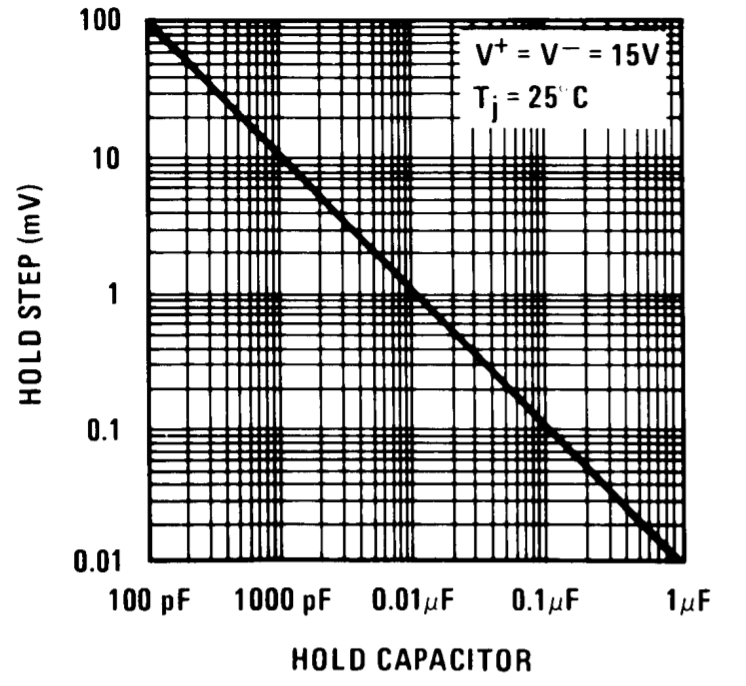
\includegraphics[width = 0.5\textwidth]{figures/hold_step_datasheet.png}
			\caption{Hold step en funci\'on de $C_H$.}
			\label{fig:syh_hold_step_datasheet}
		\end{figure}

Al igual que $V_{OS}$, el hold step $V_{HS}$ tiene que ser menor que $\frac{1}{2} LSB$ = $20mV$. Dejando un m\'argen de seguridad, se limita el valor de $V_{HS}$ a $10mV$ o menos, de forma que \[ C_H \geqslant 1nF \]
	
	
	\item\textbf{Acquisition time}
	
Como la resolucion es de 8bits, el error debe ser menor que $\frac{1}{2}$LSB = $\frac{FS}{2^9} = FS \cdot 0.02\% $. Por lo tanto, se utiliza la curva de 0.01\% de la hoja de datos (figura \ref{fig:syh_acquisition_time_datasheet} ).

Frecuencia de sampleo: $f_s = 100kHZ $ \\
Periodo de sampleo: $T_s = \frac{1}{f_s} = 10\mu s$


El sistema tiene $10\mu s$ para estar en modo \textit{sample} y en modo \textit{hold}, por lo que el tiempo de adquisici\'on hasta 0.2\% debe ser menor a $10\mu s$. De lo contrario no tendr\'ia tiempo para estar en modo sample. De la curva de 0.1\% de la figura \ref{fig:syh_acquisition_time_datasheet} se observa que para que se cumplan los requisitos anteriores se debe cumplor que \[C_H \leqslant 4nF\]

 
		\begin{figure}[H]
			\centering
			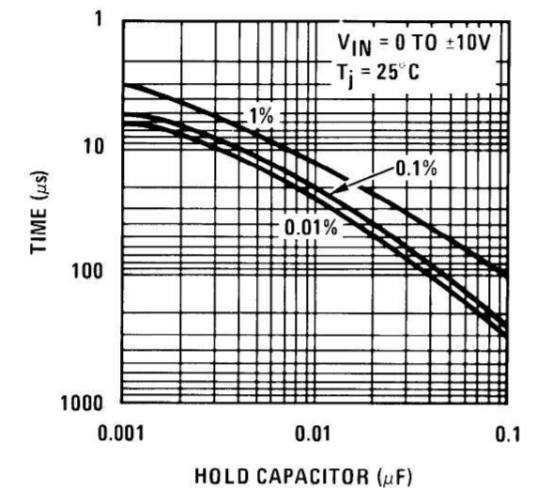
\includegraphics[width = 0.5\textwidth]{figures/acquisition_time_datasheet.png}
			\caption{Tiempo de adquisici\'on en funci\'on de $C_H$.}
			\label{fig:syh_acquisition_time_datasheet}
		\end{figure}	
		
		
		
	\item \textbf{Droop rate}
	
	El droop rate no presenta una limitaci\'on para esta aplicaci\'on en particular debido a los cortos tiempos de hold con los que se trabaja. Suponiendo que su valor es el m\'aximo presentado por el fabricante ($1V/s$), como el tiempo de \textit{hold} es menor que $10\mu s$, el m\'aximo error posible por \textit{droop} es $10\mu V$, lo cual es despreciable frente a $\frac{1}{2}$LSB = $10mV$.1
	
		\begin{figure}[H]
			\centering
			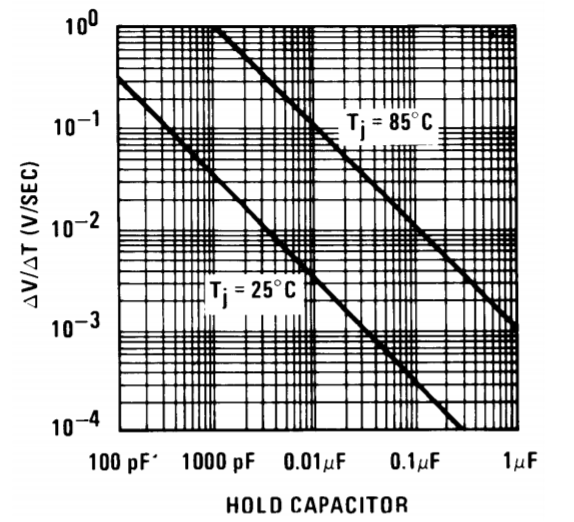
\includegraphics[width = 0.5\textwidth]{figures/droop_datasheet.png}
			\caption{Droop rate en funci\'on de $C_H$.}
		\end{figure}	
\end{itemize}

Adem\'as de las restricciones anteriores, es importante considerar que si existiera el ADC, ser\'ia conveniente que el tiempo de \textit{sample} sea lo m\'as chico posible comparado con el tiempo de \textit{hold}. Por lo tanto, se prioriza acortar lo m\'as posible el tiempo de adquisici\'on: \[C_H=1nF\]

\subsection{Tecnolog\'ia}
Uno con baja absorcion dielectrica.


\section{Duty cycle}
Se elige un duty cycle de 50\%, lo cual deja $5 \mu s$ para el modo \textit{sample} y $5 \mu s$ para el modo hold. Hay tiempo suficiente como para que se establezca la se\~nal en el modo \textit{sample} al menos al 0.1\% (con que se establezca al 0.2\% alcanzar\'ia para un ADC 8 bits). En la figura \ref{fig:syh_hold_settling_time_datasheet} se observa que el tiempo de establecimiento en modo \textit{hold} es menor a $1.4\mu s$ para el rango de temperaturas posibles de trabajo, por lo que quedar\'ian $5\mu s - 1.4 \mu s = 3.6 \mu s$ de se\~nal lo suficientemente establecida como para ser sampleada por un ADC.

		\begin{figure}[H]
			\centering
			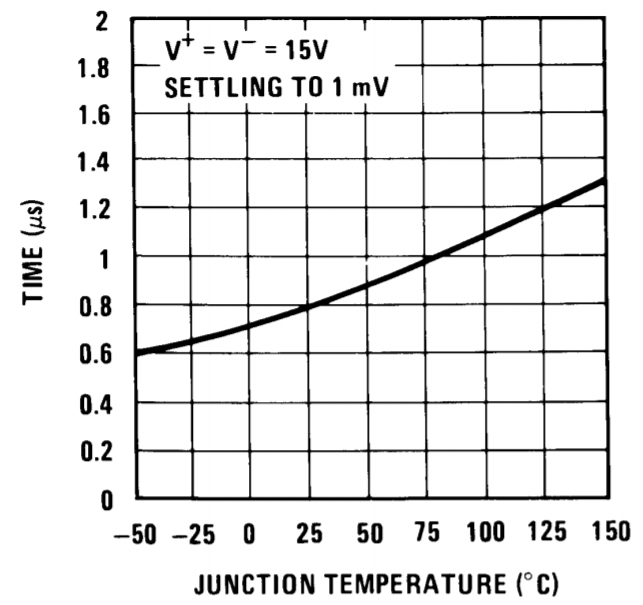
\includegraphics[width = 0.5\textwidth]{figures/hold_settling_time_datasheet.png}
			\caption{Hold settling time en funci\'on de la temperatura.}
			\label{fig:syh_hold_settling_time_datasheet}
		\end{figure}


\section{Circuito de correcci\'on de offset} \label{sec:syh_correccion_offset}

		\begin{figure}[H]
			\centering
			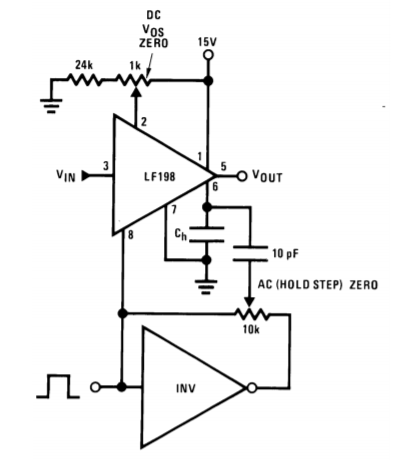
\includegraphics[width = 0.5\textwidth]{figures/offset_adjust_schematic.png}
			\caption{Circuito de correcci\'on de \textit{hold step} y de tensi\'on de offset $V_{OS}$.}
			\label{fig:syh_offset_correction_datasheet}
		\end{figure}	
		
		En la figura \ref{fig:syh_offset_correction_datasheet} se observan dos circuitos de correcci\'on. El superior es para correcci\'on de $V_{OS}$, mientras que inferior para la correcci\'on del \textit{hold step}. No se incluyen en el circuito dado que, como se mencion\'o anteriormente, la suma de estos errores es menor a $\frac{1}{2}LSB$.

\section{Simulaciones y mediciones. Comparaci\'on.}
Basado en el diagrama de la figura \ref{fig:syh_block_diagram_datasheet} de la hoja de datos, se realizo la simulaci\'on de la figura \ref{fig:syh_lt_spice} en LTSpice para contrastar con las mediciones. No es esperable que las simulaciones coincidan en todos los aspectos con todas las mediciones, ya que en muchos aspectos es ideal y en otros no:

\begin{itemize}
	\item En la simulaci\'on, la llave anal\'ogica tiene una resistencia de $1\Omega$ cuando est\'a cerrada y de $1M\Omega$ cuando est\'a abierta. Estos datos fueron asumidos dado que en la hoja de datos no est\'an especificados. Se verific\'o que al aumentar la resistencia de la llave cuando estaba cerrada, la ca\'ida de tensi\'on en el capacitor en modo \textit{hold} disminu\'ia (en el \'unico caso en que se pudo apreciar fue en el de $C_H = 1pF$ y $f_{entrada} = 8.3KHz$, ya que en los dem\'as la ca\'ida era imperceptible. Tal como fue predicho en la tabla \ref{tab:syh_droop_rate}, \'este es el caso con mayor \textit{droop-rate}, aunque el valor visto experimentalmente es mucho mayor al esperado).
	\item Al no contar con informaci\'on sobre los buffers del integrado, se usaron dos \textit{op-amps} con $A_{ol} = 100V/mV$ y $GBW = 3MHz$, e ideales en todos los dem\'as par\'ametros. En simulaciones iniciales, se parti\'o de $GBW=10MHz$. Se observ\'o que modificar este valor no manifestaba diferencias apreciables cuando $f_{entrada} = 8.3KHz$, pero s\'i cuando $f_{entrada} = 1.2MHz$. En este \'ultimo caso, al reducir $GBW$ se observa un aumento en el desfasaje entre la entrada y la salida. Comparando con la medici\'on, se estim\'o el valor $GBW = 3MHz$.
 
	\item Los modelos de los diodos, resistencias, y del capacitor son ideales.
	
\end{itemize}



\begin{figure}[H]
	\centering
	\begin{subfigure}[t]{0.45\linewidth}
		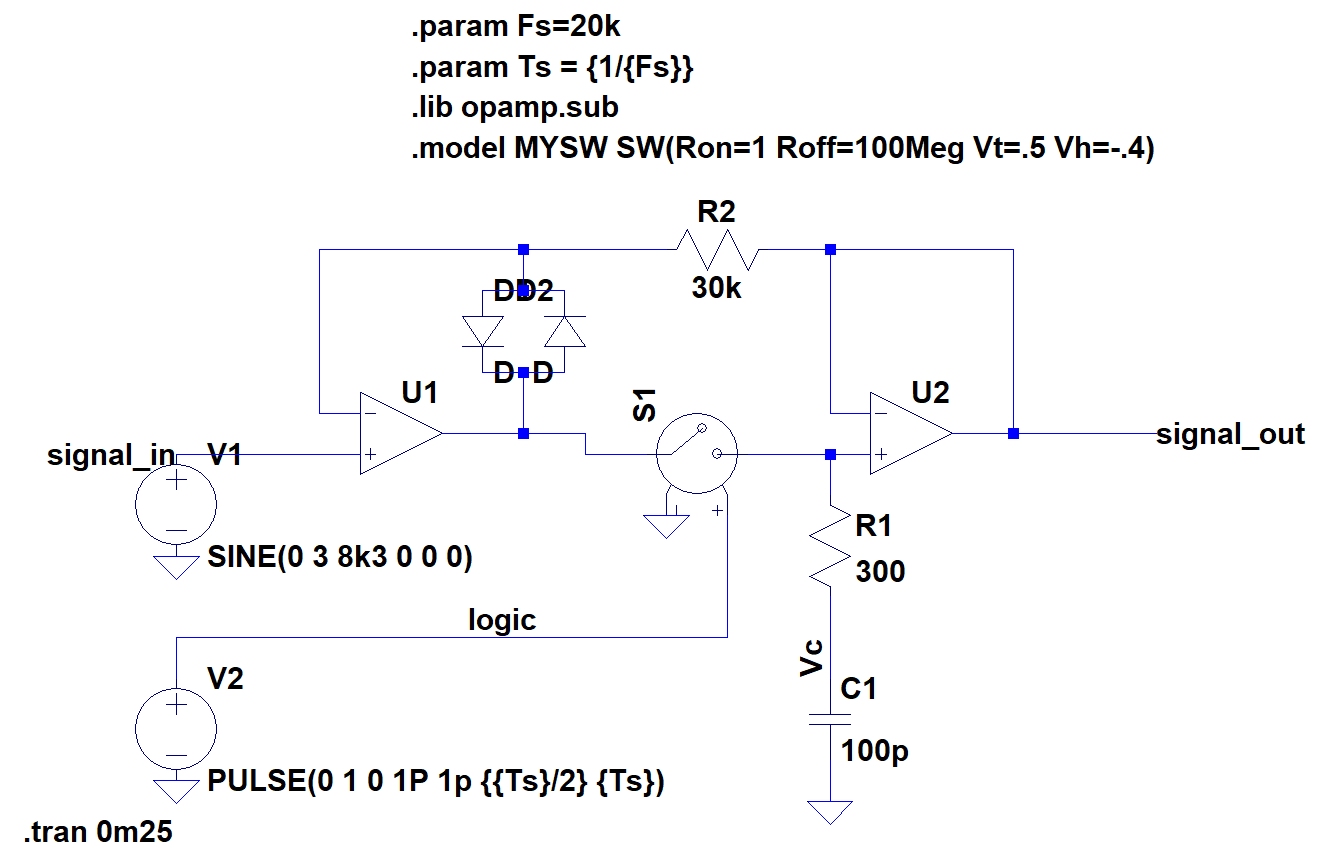
\includegraphics[width=\textwidth]{figures/ltspice_sim.png}
		\subcaption{Simulaci\'on ltSpice.}
		\label{fig:syh_lt_spice}
	\end{subfigure}
	\begin{subfigure}[t]{0.45\linewidth}
		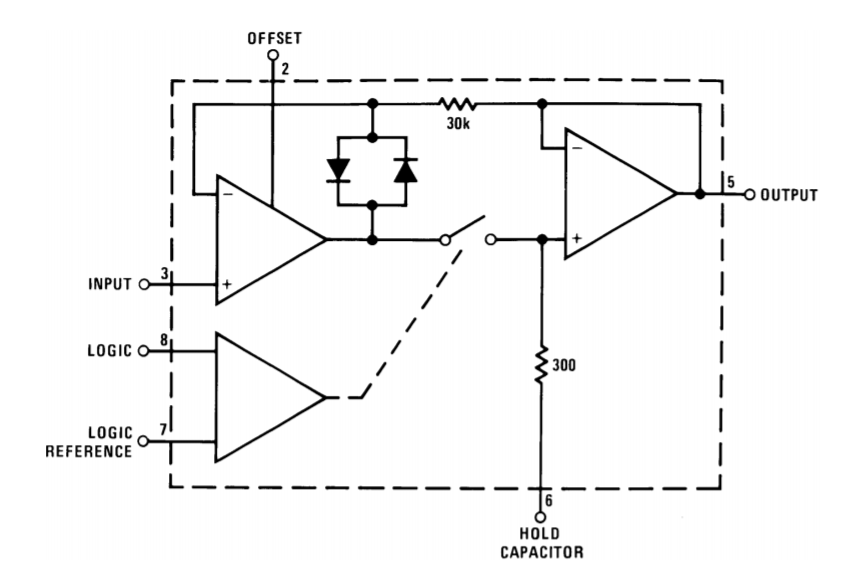
\includegraphics[width=\textwidth]{figures/block_diagram_datasheet.png}
		\subcaption{Diagrama especificado por el fabricante usado como base de la simulaci\'on. La arquitectura es lazo cerrado limitador.}
		\label{fig:syh_block_diagram_datasheet}
	\end{subfigure}
	\caption{\textit{Sample and hold}. $f_{entrada} = 1M2$, $f_{SCSH}=2M4$, $C_H = 100nF$.}
	\label{fig:syh_block_diagram_sim}
\end{figure}


Sabiendo el \textit{droop-rate} correspondiente a cada capacitor y $f_s$ se estima la p\'erdida de tensi\'on en cada periodo de \textit{hold}:
\[ \text{Droop rate} \cdot \frac{0.5}{f_s} = \Delta V\]

\begin{table}[H]
	\centering
	\begin{tabular}{|c|c|c|}
	\hline 
	 & $C_H = 100nF$ & $C_H = 100pF$ \\ 
	\hline 
	$f_s = 20KHz$ & $5.0nV $ & $7.5\mu V$ \\ 
	\hline 
	$f_s=2.4MHz$ & $42pV$ & $63nV$ \\ 
	\hline 
	\end{tabular}
	\caption{Ca\'ida de tensi\'on en modo \textit{hold} seg\'un la hoja de datos}
	\label{tab:syh_droop_rate}
\end{table}


\subsection{$f_{entrada}=1M2$, $C_H = 100nF$ } 
\label{ssec:syh_1m2_2m4_100n}
Tanto en la simulaci\'on como en la medici\'on, la tensi\'on en $C_H$ no copia a la se\~nal de entrada (\ref{fig:syh_1m2_2m4_100n}). Esto se debe al pasabajos $RC$ de primer orden formado por $C_H$ y la resistencia de $300\Omega$ con frecuencia de corte $f_0 = \frac{1}{2\pi RC} = 5.3KHz \ll f_{entrada}$. \todo{comparar las tension $C_H$ medicion simulacion y explicar por que la azul medida es como es.}

\begin{figure}[H]
	\centering
	\begin{subfigure}[t]{0.45\linewidth}
		\begin{tikzpicture}
\begin{axis}[
	xlabel = Tiempo (s),
	ylabel = Tensi\'on (V),
	width = \textwidth, 
	cycle list name = color list,
	ytick = {-5,...,5}]
\addplot table [x=x-axis, y=1, col sep=comma] {\pgfpath../mediciones/sh_1m2_2m4_n.csv};
\addplot table [x=x-axis, y=2, col sep=comma] {\pgfpath../mediciones/sh_1m2_2m4_n.csv};
\addplot table [x=x-axis, y=3, col sep=comma] {\pgfpath../mediciones/sh_1m2_2m4_n.csv};
\addplot table [x=x-axis, y=4, col sep=comma] {\pgfpath../mediciones/sh_1m2_2m4_n.csv};

\legend{Input, Output, Tensi\'on $C_H$, SCSH}
\end{axis}
\end{tikzpicture}
		\subcaption{Medici\'on.}
		\label{fig:syh_1m2_2m4_100n_med}
	\end{subfigure}
	\begin{subfigure}[t]{0.45\linewidth}
		\input{figures/syh_1M2_2M4_100n_sim.tikz}
		\subcaption{Simulaci\'on ltSpice.}
		\label{fig:syh_1m2_2m4_100n_sim}
	\end{subfigure}
	\caption{\textit{Sample and hold}. $f_{entrada} = 1M2$, $f_{SCSH}=2M4$, $C_H = 100nF$.}
	\label{fig:syh_1m2_2m4_100n}
\end{figure}

\todo[inline]{Grafico de tension en el capacitor}

%%\begin{figure}[H]
%%	\centering
%%	\begin{subfigure}[t]{0.45\linewidth}
%%		\begin{tikzpicture}
\begin{axis}[
	xlabel = Tiempo (s),
	ylabel = Tensi\'on (V),
	width = \textwidth, 
	cycle list name = color list,
	ytick = {-5,...,5}]

\addplot table [x=x-axis, y=3, col sep=comma] {\pgfpath../mediciones/sh_1m2_2m4_n.csv};

\legend{Tensi\'on $C_H$}
\end{axis}
\end{tikzpicture}
%%		\subcaption{Medici\'on.}
%%		\label{fig:syh_1m2_2m4_100n_Vc_med}
%%	\end{subfigure}
%%	\begin{subfigure}[t]{0.45\linewidth}
%%		\input{figures/syh_1M2_2M4_100n_Vc_sim.tikz}
%%		\subcaption{Simulaci\'on ltSpice.}
%%		\label{fig:syh_1m2_2m4_100n_Vc_med}
%%	\end{subfigure}
%%	\caption{Detalle de la tensi\'on en $C_H$ en el \textit{sample and hold}. $f_{entrada} = 1M2$, $f_{SCSH}=2M4$, $C_H = 100nF$.}
%%	\label{fig:syh_1m2_2m4_100n_Vc}
%%\end{figure}

\subsection{$f_{entrada}=1M2$, $C_H = 100pF$ } \label{ssec:syh_1m2_2m4_100p}
Como ya se mencion\'o, se observa un desfasaje entre la entrada y la salida, posiblemente causado por el ancho de banda limitado de los buffers. 
Tambi\'en se observa en la medici\'on un sobrepico m\'as pronunciado en la transici\'on de modo \textit{sample} a modo \textit{hold} que en cualquiera de los otros casos. 
Este efecto no pudo ser obtenido en la simulaci\'on. \todo{explicar esto, lo raro es que arranca antes del modo hold}. 
A diferencia del caso de la secci\'on \ref{ssec:syh_1m2_2m4_100n}, la tensi\'on en $C_H$ sigue a la se\~nal de entrada


\begin{figure}[H]
	\centering
	\begin{subfigure}[t]{0.45\linewidth}
		\begin{tikzpicture}
\begin{axis}[
	xlabel = Tiempo (s),
	ylabel = Tensi\'on (V),
	width = \textwidth, 
	cycle list name = color list,
	ytick = {-4,...,5},
	ymax = 3.5
	]
\addplot table [x=x-axis, y=1, col sep=comma] {\pgfpath../mediciones/sh_1m2_2m4_p.csv};
\addplot table [x=x-axis, y=2, col sep=comma] {\pgfpath../mediciones/sh_1m2_2m4_p.csv};
\addplot table [x=x-axis, y=3, col sep=comma] {\pgfpath../mediciones/sh_1m2_2m4_p.csv};
\addplot table [x=x-axis, y=4, col sep=comma] {\pgfpath../mediciones/sh_1m2_2m4_p.csv};

\legend{Input, Output, Tensi\'on $C_H$, SCSH}
\end{axis}
\end{tikzpicture}
		\subcaption{Medici\'on.}
		\label{fig:syh_1m2_2m4_100p_med}	
	\end{subfigure}
	\begin{subfigure}[t]{0.45\linewidth}
		\input{figures/syh_1M2_2M4_100p_sim.tikz}
		\subcaption{Simulaci\'on ltSpice.}
		\label{fig:syh_1m2_2m4_100p_sim}
	\end{subfigure}
	\caption{\textit{Sample and hold}. $f_{entrada} = 1M2$, $f_{SCSH}=2M4$, $C_H = 100pF$.}
	\label{fig:syh_1m2_2m4_100p}
\end{figure}

\subsection{$f_{entrada}=8.3KHz$, $C_H = 100nF$ }
Al igual que en el caso de la figura \ref{fig:syh_1m2_2m4_100n}, debido al filtro pasabajos $RC$ de primer orden, la tensi\'on en $C_H$ no puede seguir a la se\~nal de entrada en modo \textit{sample} (ver figura \ref{fig:syh_8k3_20k_100n}). Dado que el efecto se produce tambi\'en en la simulaci\'on y el modelo de capacitor usado es ideal, se puede descartar que esto sea causado por efecto de histeresis de capacitor. 

%EL ANALISIS DE ABAJO ESTA MAL
%Este fen\'omeno podr\'ia ser atribuido err\'oneamente al efecto de hist\'eresis en el capacitor debido a que se reduce al aplicar el circuito de correcci\'on de hist\'eresis propuesto en la hoja de datos (figura \ref{fig:syh_hysteresis_adjustment_datasheet}).


\begin{figure}[H]
	\centering
	\begin{subfigure}[t]{0.45\linewidth}
		\input{figures/syh_8k3_20k_100n.tikz}
		\subcaption{Medici\'on.}
		\label{fig:syh_8k3_20k_100n_med}
	\end{subfigure}
	\begin{subfigure}[t]{0.45\linewidth}
		\input{figures/syh_8k3_20k_100n_sim.tikz}
		\subcaption{Simulaci\'on ltSpice.}
		\label{fig:syh_8k3_20k_100n_sim}
	\end{subfigure}
	\caption{\textit{Sample and hold}. $f_{entrada} = 8.3KHz$, $f_{SCSH}=20KHz$, $C_H = 100nF$.}
	\label{fig:syh_8k3_20k_100n}
\end{figure}



%\begin{figure}[H]
%	\centering
%	\begin{subfigure}[t]{0.45\linewidth}
%		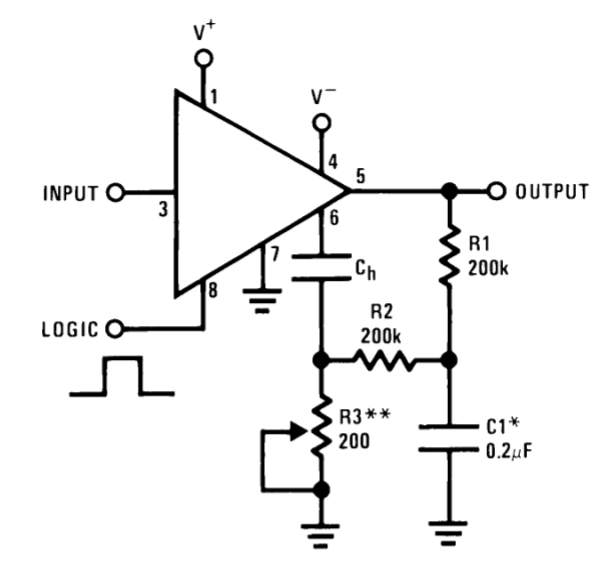
\includegraphics[width = \textwidth]{figures/hysteresis_adjust_datasheet.PNG}
%		\subcaption{Circuito propuesto por el fabricante.}
%		\label{fig:syh_hysteresis_adjustment_datasheet}
%	\end{subfigure}
%	\begin{subfigure}[t]{0.45\linewidth}
%		\input{figures/syh_8k3_20k_100n_hyst_sim.tikz}
%		\subcaption{Simulaci\'on ltSpice.}
%		\label{fig:syh_8k3_20k_100n_hyst_sim}
%	\end{subfigure}
%	\caption{Circuito de correci\'on de hist\'eresis}
%	\label{fig:syh_hysteresis_adjustment}
%\end{figure}



\subsection{$f_{entrada}=8.3KHz$, $C_H = 100pF$ }
En este caso el efecto del \textit{droop-rate} es apreciable en la medici\'on y en la simulaci\'on. Se observan sobrepicos en la transici\'on de hold a sample, al igual que en el caso con el mismo $C_H$ y mayor frecuencia (secci\'on \ref{ssec:syh_1m2_2m4_100p}) (tambi\'en en la medici\'on y en la simulaci\'on). \'Esta es la \'unica de las cuatro mediciones en las que se observa que la tensi\'on en $C_H$ en modo \textit{sample} sigue correctamente a la se\~nal de enrada. Adem\'as, es la \'unica en la que existe una diferencia constante en modo \textit{sample} entre la se\~nal de entrada y la salida (efecto no presente en la simulaci\'on). No es probable que e deba a la tensi\'on de offset ($V_{OS}$), dado que es de $150mV$, y el valor especificado como t\'ipico por el fabricante es $1mV$.

\begin{figure}[H]
	\centering
	\begin{subfigure}[t]{0.45\linewidth}
		\input{figures/syh_8k3_20k_100p.tikz}
		\subcaption{Medici\'on. La tensi\'on en $C_H$ y la se\~nal de salida est\'an pr\'acticamente superpuestas.}
	\end{subfigure}
	\begin{subfigure}[t]{0.45\linewidth}
		\input{figures/syh_8k3_20k_100p_sim.tikz}
		\subcaption{Simulaci\'on ltSpice.}
	\end{subfigure}
	\caption{\textit{Sample and hold}. $f_{entrada} = 8.3KHz$, $f_{SCSH}=20KHz$, $C_H = 100pF$.}
\end{figure}

\section{Comparaci\'on con integrado \textit{sample and hold AD585}}


\begin{center}
\begin{tabular}{|c|c|c|}
\hline 
 & LF398 & AD585 \\ 
\hline 
\hline
Arquitectura & Lazo cerrado limitador & Integrador\footnotemark \\ 
\hline 
$V_{OS}$ & $10mV$ m\'ax. ($C_H = 10nF$) & $5mV$ m\'ax. ($C_H:$ interno) \\ 
\hline 
\textit{Hold step} & $2.5mV$ m\'ax. ($C_H = 10nF$) & $3mV$ m\'ax. ($C_H:$ interno) \\ 
\hline 
\textit{Droop rate} & \begin{tabular}{c} $0.1V/s$ m\'ax. ($C_H=10nF$)\\ $1V/s$ m\'ax. ($C_H=1nF$)\end{tabular} &  $1V/s$ m\'ax. ($C_H:$ interno)\\ 
\hline 
Tiempo adquisici\'on (0.01\%)& \begin{tabular}{c} $20 \mu s$ ($C_H=10nF$)\\ $4 \mu s$ ($C_H=1nF$)\end{tabular} & $5 \mu s$ m\'ax ($C_H$: interno) \\ 
\hline 
Capacitor interno & No & S\'i ($100pF$) \\ 
\hline 
\begin{tabular}{c}
Terminal para circuito \\ de compensaci\'on de $V_{OS}$
\end{tabular} & S\'i & S\'i \\ 
\hline 
Ajuste de ganancia & No & S\'i\footnotemark \\ 
\hline 
Precio & $1.66US\$ $ & $120 US\$ $ \\ 
\hline 
\end{tabular} 
\end{center}
\footnotetext{Permite diferentes conexiones, tanto a lazo cerrado como a lazo abierto. Esto le da al usuario m\'as flexibilidad.}
\footnotetext{Esto es posible dado que el integrado permite el uso de una red de feedback externa.}
\end{document}
